\section{A Lightweight Profiler}
We design and implement a lightweight profiler, which is called LTrace, to capture the execution statistics. The design of the LTrace is introduced in the following content.

\noindent\textbf{Design Goals: }The new profiler to capture the execution statistics should address the following characteristics.
\begin{itemize}
\item \textbf{Lightweight: }The execution of the profiler consumes some resources of the cluster, which affects the execution performance of the running MapReduce jobs. In order to minimize the impact on the running MapReduce jobs, the profiler LTrace should be lightweight.
\item \textbf{Accuracy: }A MapReduce job is completed by a number of map and reduce tasks, and these tasks may execute on different machines. Due to the various performance of different machines in the cluster, the execution statistics of each task on different machine have some variances. In order to accurately capture the execution statistics of the MapReduce job, the profiler LTrace should extract the statistics of the tasks executed on the different machines accurately.
\end{itemize}

\noindent\textbf{Design and Implementation: }To realize the above design goals, we design the profiler LTrace as follows.

\begin{figure}[htbp]
\begin{center}
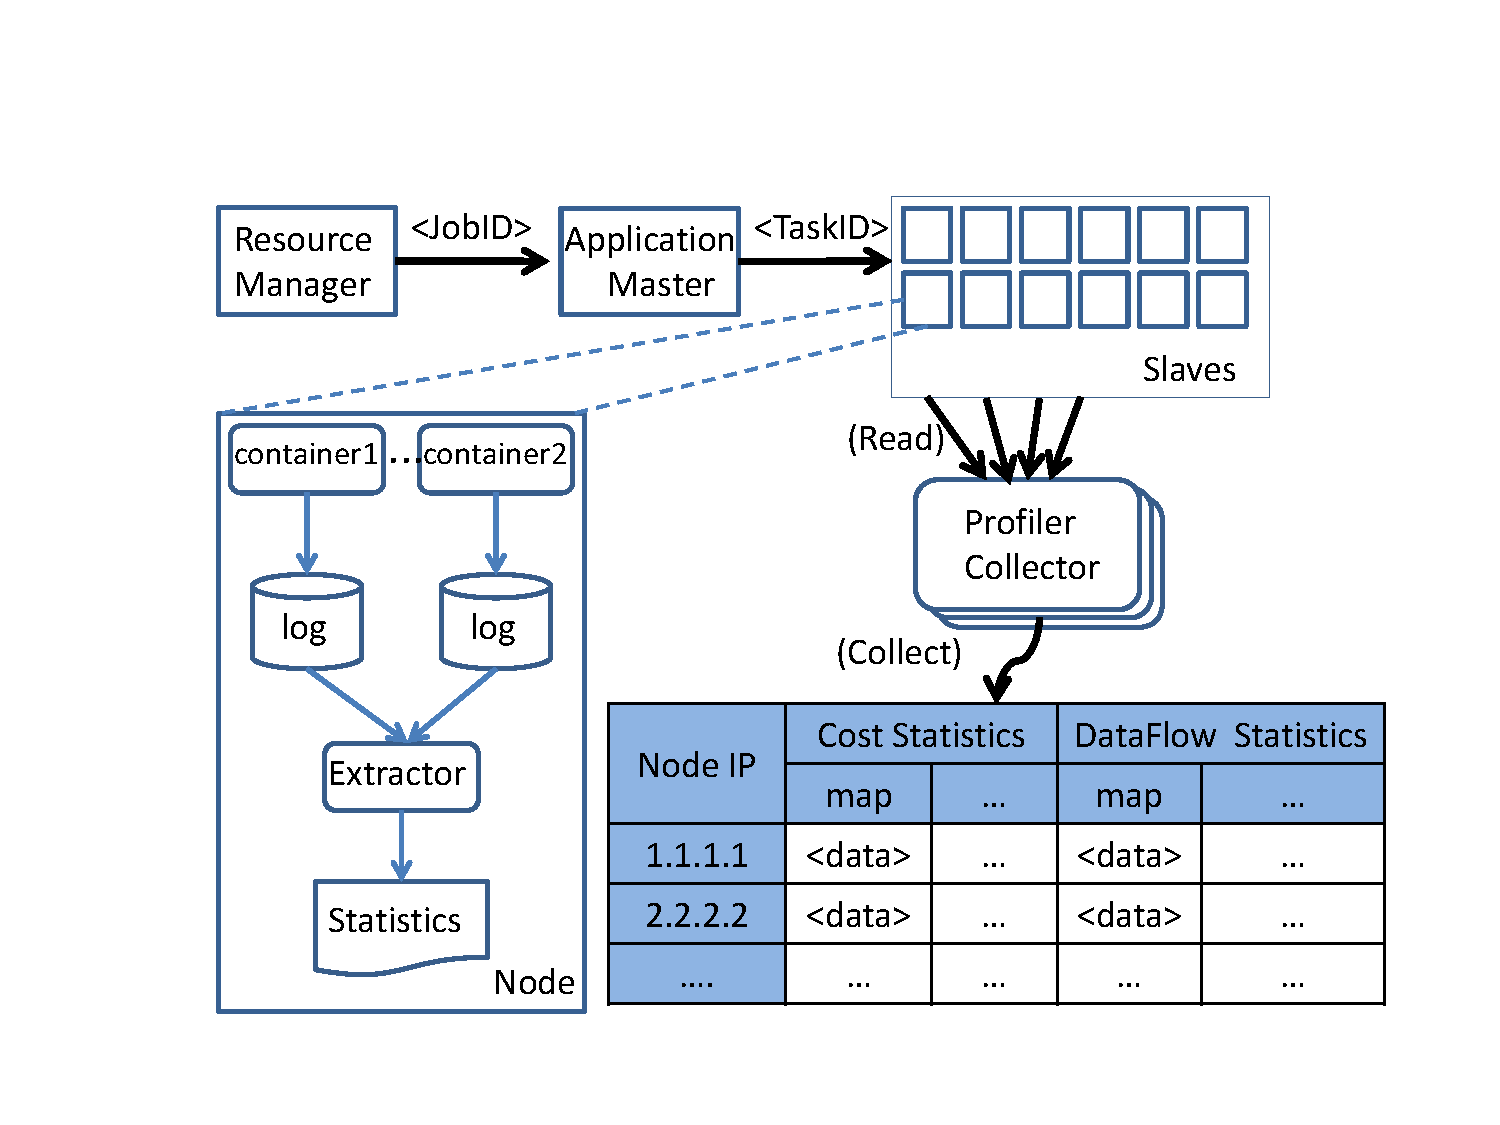
\includegraphics[height=5.5cm, width=8cm]{profiler}
\caption{The Data Flow of LTrace}
\end{center}
\end{figure}

The data flow diagram of the profiler is shown as the figure 2. In order to be a lightweight tools, the LTrace is divided into two separate parts, and these two parts are respectively designed to generate the raw data of data flow and cost when the map and reduce tasks are executing and to off-line extract the execution statistics of the MapReduce job from the raw data. The raw data of the data flow and cost is generated by means of the log system, a small number of logging statements are inserted to record the row data and printed to the local disk when the task is running. Then the log data is extracted to obtain the execution statistics when the execution of the job is complete.

There are multiple MapReduce jobs executed simultaneously on the hadoop cluster and even multiple map and reduce tasks executed simultaneously on the same machine. A MapReduce job consists of multiple map and reduce tasks, and a map or reduce task generates a log file. In order to divide these log files into different partitions that the log files of the same partition are generated by the same MapReduce job, it is essential to add a unique job id to each log. As shown the figure 2, a new MapReduce job is submitted to hadoop cluster, the resource manager allocates the resources for the new jobs  and then start the application master which schedules the execution of the map and reduce tasks for the current MapReduce job. The application master receives a unique job id from the resource manager when it starts, and a unique task id is assigned to the start-up map or reduce task. Therefore, each map or reduce task owns a unique task id, and the task id can also identify the all the tasks scheduled by the same MapReduce job. In summary, this task id if should be automatically added to the logs generated by the task.

Apache Log4j, a popular logging system, is applied in the Apache Hadoop. The Log4j provides a convenient feature: the Mapped Diagnostic Context(MDC), and this context can be used to store values that can be displayed in every log. When the process which executes the map or reduce task is started, the task id should be injected to the MDC, and all the threads and child threads can get the task id from the MDC. In order to automatically add the task id to every log, instead of manually adding the task id to each logging statement, a new layout is implemented to redefine the format of the output logs as follows: $<date, thread, taskId, message>$.

As shown in the figure 2, the Extractor, a component of the LTrace, is deployed on all the machines in the cluster, and it off-line extract the execution statistics from the raw log files. The Profiler Collector, another component of the LTrace, is deployed on the one of the machines in the cluster. This collector collects all the execution statistics extracted by the Extractor from the other machines and stores the statistics into the disk files as shown in figure 2.
